% ICASSP 2027 submission. Built with the official ICASSP paper kit:
%   spconf.sty  (ICASSP/ICIP LaTeX style)  +  IEEEbib.bst  (IEEE bibliography style)
% Page budget: 4 pages of technical content INCLUDING figures and references;
% an optional 5th page may hold references, funding acknowledgements and the
% Compliance with Ethical Standards statement only.
\documentclass{article}
\usepackage{spconf,amsmath,amssymb,graphicx,booktabs,microtype,enumitem}
\usepackage{tikz}
\usetikzlibrary{arrows.meta,positioning,fit,backgrounds,calc}
\usepackage[hidelinks]{hyperref}

\title{Knowing When Not to Match:\\Open-Set Field Alignment across ICU Databases}

\name{Anonymous submission}
\address{Affiliation withheld for anonymous review}

\begin{document}
\maketitle

\begin{abstract}

Deploying a physiological monitoring model across hospitals requires aligning the
signal channels of one intensive-care database to those of another, a step still done
by hand. We show that a frozen language model reading only data dictionaries and
training-split aggregate statistics---never patient trajectories---ranks the correct
target concept first for $88$--$97\%$ of mappable fields across three ICU databases.
The binding constraint is elsewhere: among fields recorded for at least $5\%$ of stays,
$77\%$ match no concept in a $138$-concept catalogue, and over-assignment accounts for
$90.5\%$ and $93.0\%$ of errors on two of three databases. We therefore read
deterministic unit, type and specimen compatibility as \emph{abstention evidence}
rather than as a re-ranking filter. Holding the penalty, its weight, the candidates, the
calibration split and the test fields fixed and varying only what consumes the signal,
re-ranking and rejection cost $2.6$--$10.2$ Recall@1 points for no consistent detection
gain, whereas abstention improves open-set AUROC by $5.7$ points on two databases
(paired bootstrap $95\%$ CI excluding zero) and $0.7$ on the third. Two blinded
independent experts ($\kappa{=}0.952$) put the error rate of the strata they reviewed at
$3.96\%$, and applying every correction leaves the result intact. We release $710$ field--concept pairs over $135$ concepts with per-pair
evidence provenance and $2{,}428$ adjudicated \textsc{unknown} fields.
\end{abstract}

\begin{keywords}
schema alignment, open-set recognition, selective prediction, physiological time
series, clinical databases
\end{keywords}

\section{Introduction}

Deploying a physiological monitoring model across hospitals begins with a step no model
can skip: deciding which channel is which. \texttt{itemid 220045} in one intensive-care
database and \texttt{Vital Signs|Heart Rate} in another carry the same signal; a third
field named \texttt{Heart Rate} in a nurse-charting table does not. Of the $135$ concepts
we align, $63$ are continuously monitored channels, and eICU's periodic vitals table
alone holds $5.5\times10^{8}$ samples of them. A mis-assigned channel is a signal-level
defect: a temperature series concatenated across Celsius and Fahrenheit sources, or an
arterial line merged with a cuff, corrupts every filter computed downstream.

Existing approaches to this alignment fall into two families. \emph{Curated dictionaries}
map each database by hand into a shared concept
vocabulary~\cite{ricu,ohdsi,mimiccode}. They are accurate but partial by construction:
\texttt{ricu} maps $119$ concepts across five databases and states that its dictionary is
not comprehensive, and the three public expert mappings we use agree with one another at
pairwise Jaccard $0.29$--$0.42$. \emph{Automatic schema
matching} instead learns or prompts the correspondence~\cite{rahm2001,llmatch,bdiviz}.
Both families share an assumption that the clinical setting violates: that every source
attribute has a target. They also assume the metadata a matcher would use is present,
whereas four eICU tables covering $319$ fields and $7.3\times10^{8}$ rows carry no unit
column at all.

Given this, one expects automatic alignment to be hard. It is not---at least not the part
usually measured. A frozen language model prompted with the schema-matching template of
LLMatch~\cite{llmatch}, shown only dictionary labels and training-split aggregates, ranks
the correct concept first for $95.9$, $97.3$ and $88.2\%$ of mappable fields on MIMIC-IV,
MIMIC-III (CareVue) and eICU. The difficulty lies in the complement: of the fields
recorded for at least $5\%$ of stays, $77.1\%$ belong to no concept in our $138$-concept
catalogue---site-local assays, device settings, free-text flags, nursing observations.
Precision is consequently only $69$--$85\%$, and an error decomposition attributes
$90.5\%$ and $93.0\%$ of errors on MIMIC-IV and CareVue to assigning a concept to a field
that has none. The binding problem is abstention, not ranking.

Abstention is well studied as selective prediction and open-set
recognition~\cite{selective,openset,msp}, but there the thresholded confidence comes from
the classifier's own output distribution. A generative matcher has no such distribution:
it emits an accept/reject decision with no graded score. A natural substitute is to
reject implausible matches with deterministic compatibility rules---a field in
\textsc{mg/dL} cannot realise a concept in \textsc{mmHg}; a field assayed on ascites
cannot realise a serum concept. Used that way the rules \emph{lose}, costing
$2.6$--$10.2$ Recall@1 points for no consistent detection gain, because the matcher
already respects them in $99.3$--$100\%$ of accepted matches. Motivated by this
observation, we move the same signal to a different position in the pipeline: rather than
deciding \emph{which} concept a field takes, the checks score how much evidence
contradicts the match already made, and that score becomes the abstention criterion.

Our main contributions are three folds: (1) We propose reading deterministic unit, data
type and specimen compatibility as \emph{abstention evidence} rather than as a
re-ranking filter, which improves open-set AUROC by $5.7$ points on two of three
databases without changing which concept is proposed, and we isolate the effect with a
controlled comparison that holds the penalty, its weight, the candidates and the
calibration split fixed and varies only what consumes the signal. (2) We release a
three-database field-level reference standard for open-set alignment---$710$
field--concept pairs covering $135$ of $138$ catalogue concepts, and $2{,}428$ adjudicated
\textsc{unknown} fields drawn from real schemas rather than constructed as
negatives---validated by two blinded independent human experts ($\kappa{=}0.952$).
(3) We show the effect replicates across three language-model families and quantify what
alignment quality is worth downstream, in a zero-shot cross-database transfer of a
$24$-channel physiological time-series model.

\begin{figure*}[t]
\centering
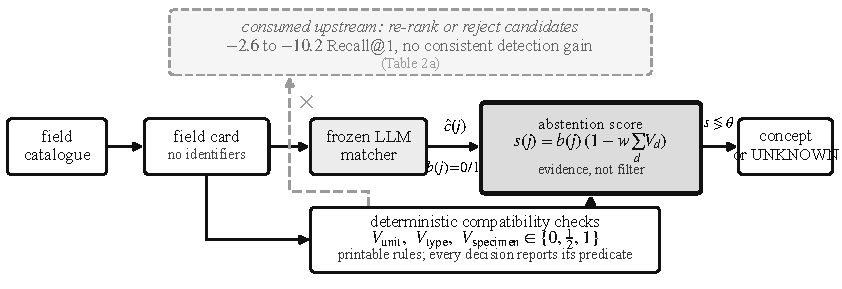
\includegraphics[width=0.88\textwidth]{figures/method.pdf}
\caption{The overall architecture of the proposed method. Deterministic compatibility
checks are read as evidence about a match the frozen matcher has already made: they
discount the confidence $b(j)$ attached to $\hat{c}(j)$ and never change which concept is
proposed. Consuming the identical penalty one step earlier---to re-rank or reject
candidates---costs $2.6$--$10.2$ Recall@1 points for no consistent detection gain
(Table~\ref{tab:ablate}a).}
\label{fig:arch}
\end{figure*}

\section{Method}
\label{sec:method}


Fig.~\ref{fig:arch} shows an overview of the proposed method. A field is first rendered
into a textual field card, which a frozen language model maps to a candidate concept;
four deterministic predicates then compare the field against a representative of that
concept, and their total discounts the matcher's confidence to give an abstention score.

\subsection{Field Cards}

Let $\mathcal{C}$ be a catalogue of unified clinical concepts and $j$ a field of a target
database. We render $j$ into a fixed template holding its dictionary label and
abbreviation, source table, category, inferred data type, modal observed unit,
training-split $1$st/$50$th/$99$th value percentiles, observations per stay and missing
rate. Units are recovered from observed values rather than read from the dictionary,
because dictionaries usually lack them: $85.3\%$ of MIMIC-IV \texttt{chartevents}
dictionary entries carry no unit.

A runtime assertion forbids any numeric primary key---item identifier, laboratory
identifier, or stay, admission and subject keys---from appearing in a card. This matters
because \texttt{mimic-code}~\cite{mimiccode} is a widely mirrored public repository, so a
card carrying an identifier would let a language model retrieve a memorised crosswalk
instead of reading the field; Sec.~\ref{sec:ablation} tests whether it does. No patient
trajectory enters the card.

\subsection{Deterministic Compatibility Checks}

For a field $j$ and a candidate concept $c$ we evaluate four predicates, each returning
$V_d(j,c)\in\{0,\tfrac12,1\}$ for compatible, undecidable and incompatible. Every
predicate is printable, and each decision is reported together with the rule that
produced it.

\noindent\textbf{Unit.}
$V_{\mathrm{unit}}$ performs dimensional analysis against a conversion table in which
every row cites a public source. Exactly convertible pairs
(\textsc{mEq/L}$\leftrightarrow$\textsc{mmol/L} for monovalent ions) are compatible;
dimension mismatches are incompatible; a missing unit on either side is undecidable.

\noindent\textbf{Data type.}
$V_{\mathrm{type}}$ returns $1$ only when \emph{both} sides' types are
dictionary-declared, and $\tfrac12$ if either is inferred. The distinction is not
cosmetic: before it was introduced, $23$ of $34$ erroneous rejections on reference pairs
were numeric fields stored as text and inferred to be categorical. eICU declares no
parameter types, so all of its type conflicts are undecidable by construction.

\noindent\textbf{Specimen.}
$V_{\mathrm{specimen}}$ returns $1$ for distinct specimen types. It is the only signal
separating \texttt{Albumin} (blood) from \texttt{Albumin, Ascites}: identical names,
identical \textsc{g/dL} units, different analyte.

\noindent\textbf{Provenance.}
$V_{\mathrm{prov}}$ returns $1$ for conflicting measurement methods and $\tfrac12$ for
conflicting table families. A concept is not bound to one source table, so in
field-to-concept matching this predicate is weak by construction; the calibration of
Sec.~\ref{sec:calib} discards it.

\subsection{Abstention Score}

Let $\hat{c}(j)=\arg\max_{c\in\mathcal{C}} f(j,c)$ be the matcher's top candidate and
$b(j)$ its own confidence. A generative matcher emits a decision rather than a score, so
$b(j)\in\{0,1\}$: it is $0$ when the matcher returns no concept for $j$ and $1$
otherwise. For a ranking matcher $b(j)$ is instead the top-$1$ cosine similarity. We
score
\begin{equation}
s(j) \;=\; b(j)\Bigl(1 - w\!\!\sum_{d\in\mathcal{D}}\!\! V_d\bigl(j,\hat{c}(j)\bigr)\Bigr),
\label{eq:abstain}
\end{equation}
where $\mathcal{D}$ is the selected subset of predicates and $w$ the penalty weight, and
we declare
\begin{equation}
\hat{y}(j) \;=\;
\begin{cases}
\hat{c}(j), & s(j) \ge \theta,\\[2pt]
\textsc{unknown}, & s(j) < \theta .
\end{cases}
\label{eq:decide}
\end{equation}
The checks never alter $\hat{c}(j)$. They only discount the confidence attached to it,
which is what distinguishes Eq.~\eqref{eq:abstain} from applying the same predicates to
filter candidates before $\hat{c}(j)$ is formed.

\subsection{Calibration}
\label{sec:calib}

$\mathcal{D}$, $w$ and $\theta$ are selected on the MIMIC-IV validation split
($62$ fields, $24$ positives) over $15$ dimension subsets $\times$ $4$ weights, and are
never refitted on the reported domains or per model. The selection returns
$\mathcal{D}=\{\mathrm{unit},\mathrm{type},\mathrm{specimen}\}$ and $w{=}0.1$, dropping
$V_{\mathrm{prov}}$ in agreement with the ablation of Sec.~\ref{sec:ablation}.

The weight must be read against the spread of the confidence it discounts. For
cosine-ranked candidates the top-$1$/top-$2$ margin has median $0.068$, so $w{=}1$ makes
a single unit conflict worth seven times the gap between the two best candidates and
collapses precision from $83.6$ to $51.5$. Any reimplementation that inherits an unscaled
penalty reproduces that collapse rather than the result reported here.

\section{Experiments}
\label{sec:exp}

\begin{table*}[t]
\centering
\caption{Field alignment and open-set detection. All rows are evaluated on \emph{identical} field sets (MIMIC-IV test split, CareVue and eICU in full); $n$ fields\,/\,mappable are $132/49$, $696/296$, $244/152$. R@1 is Recall@1 over mappable fields and is blind to the abstention decision; P is precision of the top-1 assignment; AUC is open-set AUROC. $\Delta$ compares each matcher with and without the checks, with a \emph{paired} bootstrap 95\% CI over field indices ($B{=}2000$). Thresholds are fitted on the MIMIC-IV validation split only and never refitted per model.}
\label{tab:main}
\scriptsize
\setlength{\tabcolsep}{3pt}
\begin{tabular}{@{}l rrr l rrr l rrr l@{}}
\toprule
& \multicolumn{4}{c}{MIMIC-IV} & \multicolumn{4}{c}{CareVue} & \multicolumn{4}{c}{eICU} \\
\cmidrule(lr){2-5}\cmidrule(lr){6-9}\cmidrule(lr){10-13}
Matcher & R@1 & P & AUC & $\Delta$AUC\,[95\% CI] & R@1 & P & AUC & $\Delta$AUC\,[95\% CI] & R@1 & P & AUC & $\Delta$AUC\,[95\% CI] \\
\midrule
\multicolumn{13}{@{}l}{\emph{(a) non-semantic}}\\
Exact / normalized name & 36.7 & 100.0 & 68.4 & -- & 37.2 & 94.0 & 68.3 & -- & 44.1 & 98.5 & 72.4 & -- \\
Ontology only (LOINC) & 26.5 & 100.0 & 63.3 & -- & 24.7 & 100.0 & 62.3 & -- & 0.0 & 0.0 & 50.0 & -- \\
\multicolumn{13}{@{}l}{\emph{(b) frozen encoders}}\\
MiniLM-L6, 23\,M & 49.0 & 82.8 & 91.1 & -- & 62.2 & 86.8 & 90.0 & -- & 44.1 & 75.3 & 73.1 & -- \\
SapBERT, 110\,M (biomedical) & 67.3 & 91.7 & 93.4 & -- & 70.6 & 83.6 & 92.5 & -- & 57.9 & 79.3 & 80.7 & -- \\
\quad + checks as abstention & 67.3 & 91.7 & 92.4 & -- & 70.6 & 83.6 & 90.3 & -- & 57.9 & 79.3 & 79.8 & -- \\
\multicolumn{13}{@{}l}{\emph{(c) frozen LLM matchers}}\\
\textsc{gpt-4.1} (OpenAI) & 95.9 & 69.1 & 91.0 & -- & 97.3 & 72.0 & 87.9 & -- & 88.2 & 85.3 & 84.4 & -- \\
\quad + checks (\textbf{ours}) & \textbf{95.9} & \textbf{69.1} & \textbf{96.6} & \textbf{5.7\,[2.7,\,9.0]} & \textbf{97.3} & \textbf{72.0} & \textbf{93.6} & \textbf{5.7\,[4.1,\,7.2]} & \textbf{88.2} & \textbf{85.3} & \textbf{85.0} & \textbf{0.7\,[-1.5,\,2.8]} \\
\textsc{deepseek-v3.2} & 95.9 & 60.3 & 85.8 & -- & 98.0 & 68.9 & 85.9 & -- & 88.2 & 68.4 & 75.3 & -- \\
\quad + checks (\textbf{ours}) & \textbf{95.9} & \textbf{60.3} & \textbf{95.3} & \textbf{9.5\,[5.8,\,13.8]} & \textbf{98.0} & \textbf{68.9} & \textbf{93.1} & \textbf{7.2\,[5.6,\,9.0]} & \textbf{88.2} & \textbf{68.4} & \textbf{79.3} & \textbf{4.0\,[0.9,\,7.2]} \\
\textsc{gemini-2.5-pro} (Google) & 95.9 & 65.3 & 87.3 & -- & 97.6 & 70.2 & 88.0 & -- & 73.0 & 79.9 & 78.8 & -- \\
\quad + checks (\textbf{ours}) & \textbf{95.9} & \textbf{65.3} & \textbf{96.2} & \textbf{8.9\,[5.2,\,13.2]} & \textbf{97.6} & \textbf{70.2} & \textbf{95.0} & \textbf{7.1\,[5.3,\,8.8]} & \textbf{73.0} & \textbf{79.9} & \textbf{80.4} & \textbf{1.6\,[-0.6,\,4.0]} \\
\bottomrule
\end{tabular}
\vspace{-4pt}
\end{table*}


\subsection{Datasets and implementation details}
\label{sec:data}

\noindent\textbf{Databases.}
We align fields from MIMIC-IV v3.1~\cite{mimiciv}, the CareVue subset of
MIMIC-III v1.4~\cite{mimiciii} and eICU-CRD v2.0~\cite{eicu}, each restricted to a
patient's first ICU stay of at least $24$\,h ($51{,}838$, $19{,}112$ and $110{,}257$
stays). MIMIC-IV is the source domain on which every statistic and threshold is fitted.
We use the CareVue subset rather than all of MIMIC-III to limit identity-level
correspondence with MIMIC-IV; $661$ of its $3{,}545$ \texttt{chartevents} fields
nonetheless carry MIMIC-IV-range identifiers, and restricting the evaluation to
CareVue-era identifiers leaves the main effect at $+5.2$ AUROC ($95\%$ CI
$[+3.7,+6.9]$) against $+5.7$ on the full set, so shared identifiers are not carrying the
result. eICU is the hardest of the three: no item dictionary, no declared types, and no
unit column in four of its tables.

\noindent\textbf{Reference standard.}
Two independently prompted model instances, given a concept-first and a
conservative-first protocol, labelled every field recorded for at least $5\%$ of stays;
disagreements went to a third arbitrating instance. This yields $710$ field--concept
pairs ($246$/$304$/$160$ by database) covering $135$ of the $138$ catalogue concepts,
$86$ of them present in all three databases, and $2{,}428$ fields adjudicated
\textsc{unknown}; three catalogue concepts have no field in any database. Agreement
between the two instances is $0.9855$ ($\kappa{=}0.967$), but they share a pretraining
prior, so that measures protocol reproducibility rather than label validity; for validity
we rely on the blinded human review of Sec.~\ref{sec:expert}. Each pair carries its
evidence provenance: $217$ ($31\%$) rest on evidence not involving a language model,
$159$ of them from agreement among three public expert mappings. Of the $1{,}685$
high-coverage fields reviewed in the first round, $368$ ($21.8\%$) received a concept,
$1{,}299$ ($77.1\%$) were adjudicated \textsc{unknown} and $18$ remained unsure; the
negatives are therefore real schema entries, not constructed distractors.

\noindent\textbf{Evaluation sets and metrics.}
Fields are split by a hash of the field key into train, validation and test, so
calibration and reporting never share one. Each evaluation set holds that database's mappable fields plus
up to its $400$ highest-volume \textsc{unknown} fields, giving $132/49$, $696/296$ and
$244/152$ fields\,/\,mappable after the split. Each concept is represented by the
MIMIC-IV field with the most observations, so representatives come only from the source
domain. Recall@1 is computed over mappable fields only and is \emph{blind to the
abstention decision}: a method changing only the abstention score leaves it unchanged by
construction, so it measures what abstention costs the candidate ranking, not what it
costs end to end. Open-set AUROC ranks all fields by the abstention score. Thresholds are
fitted per method on the MIMIC-IV validation split.

\noindent\textbf{Matchers.}
The frozen LLM matcher is \texttt{gpt-4.1} at temperature $0$, prompted with the LLMatch
column-matching template verbatim (SHA-256 prefix \texttt{b4c100e7}) and queried in
August 2026; the adjudicating annotators are Claude instances, a distinct family. We
additionally run \texttt{deepseek-v3.2} and \texttt{gemini-2.5-pro} under an identical
prompt, temperature and abstention configuration. Every model alias, endpoint, query
date, prompt and completion is released.

\subsection{Comparison with baselines and across model families}

Table~\ref{tab:main} reports all matchers on identical field sets. Exact name matching
reaches $36.7$--$44.1$ Recall@1 but fires on only $13.6$--$27.9\%$ of fields;
ontology-only matching through recovered LOINC codes~\cite{loinc} returns \emph{exactly}
zero on eICU, which carries no standard vocabulary codes. A biomedical
encoder~\cite{sapbert} beats a general one~\cite{cpack} at equal size.

Adding the checks as abstention evidence leaves the matcher's decisions untouched and
raises open-set AUROC from $90.96$ to $96.64$ on MIMIC-IV, $87.93$ to $93.57$ on CareVue
and $84.39$ to $85.04$ on eICU. Because both scores come from the same fields, the
appropriate test is a paired bootstrap over field indices, not a comparison of marginal
intervals: over $B{=}2000$ resamples the paired $95\%$ CIs exclude zero on the first two
($\hat p(\Delta\le 0)<10^{-3}$) and not the third. A biomedical encoder's cosine is itself
a competitive detector despite ranking the correct concept first far less often; our score
is highest on all three but its margin over that encoder falls inside the marginal
intervals on two, so we defend the paired within-matcher gain.

Across the nine (model, database) cells, Recall@1 is essentially invariant on the two
MIMIC databases ($95.9$ for all three families on MIMIC-IV, $97.3$--$98.0$ on CareVue),
and seven of the nine cells are individually significant. Descriptively the gain tracks
the matcher's precision (Pearson $r{=}-0.92$), from $+9.5$ at precision $60.3$ to $+0.7$
at $85.4$; nine post-hoc, non-independent cells cannot establish that relation and we
offer it as exploratory. It is nonetheless consistent with a reading of the eICU result
other than absent metadata: there \texttt{gpt-4.1} attains its \emph{highest} precision
($85.4$), leaving little to correct, whereas \texttt{deepseek-v3.2} on the same database
and the same absent metadata reaches precision $68.4$ and gains $+3.97$ ($p{=}0.005$).

\subsection{Ablation studies}
\label{sec:ablation}

\begin{table*}[t]
\centering
\caption{The same graded penalty $w\sum_d V_d$, evaluated two ways. (a) Consumed three ways---weight, dimensions, candidates, calibration split and test fields held fixed, only the consumer varies; $\Delta$ is against the matcher's own abstention, with paired bootstrap 95\% CIs. (b) $\Delta$AUROC of each dimension subset used as abstention evidence, on the same matcher and fields.}
\label{tab:ablate}
\footnotesize
\setlength{\tabcolsep}{4pt}
\begin{tabular}{@{}l rr l rr l rr l@{}}
\toprule
& \multicolumn{3}{c}{MIMIC-IV} & \multicolumn{3}{c}{CareVue} & \multicolumn{3}{c}{eICU} \\
\cmidrule(lr){2-4}\cmidrule(lr){5-7}\cmidrule(lr){8-10}
& $\Delta$R@1 & $\Delta$AUC & 95\% CI & $\Delta$R@1 & $\Delta$AUC & 95\% CI & $\Delta$R@1 & $\Delta$AUC & 95\% CI \\
\midrule
\multicolumn{10}{@{}l}{\emph{(a) consumer of the penalty}}\\
re-rank candidates & -4.1 & -0.5 & [-1.3,\,0.0] & -4.0 & 0.3 & [-0.3,\,1.1] & -2.6 & -0.4 & [-0.8,\,-0.1] \\
reject candidates & -10.2 & -1.2 & [-5.7,\,3.0] & -7.1 & 2.7 & [0.5,\,5.0] & -5.3 & -1.9 & [-4.4,\,0.6] \\
\textbf{abstain (ours)} & \textbf{0.0} & \textbf{5.7} & \textbf{[2.7,\,9.0]} & \textbf{0.0} & \textbf{5.7} & \textbf{[4.0,\,7.2]} & \textbf{0.0} & \textbf{0.7} & \textbf{[-1.5,\,2.8]} \\
\addlinespace[2pt]
\midrule
\multicolumn{10}{@{}l}{\emph{(b) dimensions used as abstention evidence ($\Delta$AUROC)}}\\
unit only &  & 5.3 & [93.3,\,98.6] &  & 3.2 & [88.9,\,93.2] &  & -0.7 & [77.5,\,88.3] \\
data type only &  & 1.3 & [87.9,\,95.9] &  & 4.5 & [90.5,\,94.0] &  & 0.1 & [79.2,\,89.0] \\
specimen only &  & 2.8 & [90.5,\,96.5] &  & 3.1 & [89.1,\,92.9] &  & 1.8 & [81.1,\,90.4] \\
provenance only &  & -1.8 & [83.7,\,94.2] &  & -2.3 & [82.8,\,88.1] &  & -1.1 & [77.6,\,88.2] \\
all four &  & 3.9 & [91.2,\,97.7] &  & 3.8 & [89.5,\,93.5] &  & 0.0 & [78.7,\,88.9] \\
\textbf{unit + type + specimen (ours)} &  & \textbf{5.7} & \textbf{[93.8,\,98.6]} &  & \textbf{5.7} & \textbf{[91.8,\,95.3]} &  & \textbf{0.7} & \textbf{[79.2,\,89.5]} \\
\bottomrule
\end{tabular}
\vspace{-4pt}
\end{table*}


\noindent\textbf{Where the penalty is consumed.}
Table~\ref{tab:ablate}(a) holds the penalty $w\sum_d V_d$, its weight, the dimensions,
the candidates and the calibration split fixed and varies only what consumes it, so the
comparison isolates placement rather than confounding it with a switch from a graded
penalty to a binary veto. Reordering the candidates by the penalty---removing
nothing---already costs $2.6$--$4.1$ Recall@1 points and moves detection by at most half a
point; thresholding it to reject candidates costs $5.3$--$10.2$ points and helps detection
on one database only; also rejecting on the undecidable value $V_d{=}\tfrac12$ removes
$69$--$81$ points, since ``we cannot tell'' is the common case in these schemas. The same
numbers, read as evidence about a match left in place, gain $5.7$ points twice.

\noindent\textbf{Which dimensions matter.}
Used alone, unit dominates on MIMIC-IV, data type on CareVue and specimen on eICU, while
provenance alone harms all three (Table~\ref{tab:ablate}b); the selected subset excluding
it beats all four together everywhere. Applying the same evidence to the biomedical
encoder, whose cosine is already graded, changes AUROC by $-0.0$, $-1.9$ and $-1.2$ even
after re-selecting $\mathcal{D}$ and $w$ for it on the same validation split: the evidence
pays where the matcher supplies no confidence of its own, and not elsewhere.

\noindent\textbf{Operating point.}
At a threshold locked per method on the validation split, detection of unmappable fields
improves on all three ($81.9\to 86.8$, $78.0\to 90.3$, $79.4\to 81.5$) while mapping
$F_1$ improves on CareVue and declines on the other two: the method trades recall on
mappable fields for detection of unmappable ones.

\noindent\textbf{Controls.}
Adding the raw item identifier to the card leaves Recall@1 unchanged to the digit while
precision \emph{falls} by $4.7$ and $2.7$ points, so the matcher is not retrieving a
memorised crosswalk. Recall@1 on reference pairs that never involved a language model
($100.0$, $98.0$, $100.0$) exceeds that on adjudicated pairs ($94.6$, $96.9$, $84.3$),
where contamination would predict the reverse.

\subsection{Blinded expert validation}
\label{sec:expert}

Two independent human annotators---an intensive-care clinician and a clinical-data
engineer---relabelled a blinded sample of $198$ fields carrying no model answer, stratum
label or identifier, over-sampling failure-prone regions: \textsc{unknown} verdicts on
high-coverage fields ($70$), positives from model adjudication only ($50$), arbitrated
disagreements ($30$), check-flagged positives ($28$), non-model-evidence positives ($20$).
Between them Cohen's $\kappa$ is $0.952$ ($n{=}196$, chance agreement $0.260$), and
$0.939$ for the mappable-versus-\textsc{unknown} decision alone. Counting an error only
where \emph{both} contradict the reference standard, the stratum-weighted error rate over
the $1{,}877$ fields these strata cover---not over the standard as a whole---is $3.96\%$
($95\%$ CI $2.0$--$7.7$); the \textsc{unknown} verdicts on which the $77.1\%$ figure rests
are disputed in $1$ of $70$ cases, the fields on which our checks fire in $0$ of $28$.
Rebuilding the standard with every correction applied leaves the result intact
($\Delta$AUROC $+5.68$, $+5.47$, $+0.65$).

Two findings run against expectation. The stratum we treated as the trustworthy
control---positives inherited from three public expert mappings---is the \emph{least}
reliable ($20\%$ disputed), because those mappings themselves conflate point-of-care with
laboratory glucose. And six of the nine confirmed errors are measurement-method confusions
(point-of-care versus laboratory glucose, ventilator set rate versus measured respiratory
rate, arterial \textsc{sao}$_2$ versus pulse oximetry): the distinction
$V_{\mathrm{prov}}$ was meant to capture, discarded because our table-family
implementation reduced detection. A deterministic method predicate flags all six but also
fires on $8\%$ of correct pairs, because the catalogue is method-agnostic---one
\texttt{sbp}, not an invasive and a cuff variant---so our validation split never selects
it. The residual errors are a property of the target vocabulary's granularity, not of the
matcher. All six are cases where the matcher assigned a concept to a field the experts
call \textsc{unknown}: over-assignment, confirmed blind.

\subsection{Downstream cross-database transfer}
\label{sec:transfer}

\begin{table}[t]
\centering
\caption{Zero-shot cross-database transfer of a 24-channel physiological time-series model trained on MIMIC-IV (validation AUROC $84.20\pm0.12$), as a function of how target fields are mapped onto channels. Mortality AUROC, mean$\pm$sd over five seeds; $c$ = channels receiving data. The last row is a patient-level paired bootstrap of the abstention effect.}
\label{tab:transfer}
\scriptsize
\setlength{\tabcolsep}{3pt}
\begin{tabular}{@{}l cc cc@{}}
\toprule
& \multicolumn{2}{c}{CareVue ($n{=}19{,}112$)} & \multicolumn{2}{c}{eICU ($n{=}110{,}257$)} \\
\cmidrule(lr){2-3}\cmidrule(lr){4-5}
Field alignment & AUROC & $c$ & AUROC & $c$ \\
\midrule
reference (adjudicated) & 74.5\,$\pm$\,1.3 & 24 & 70.4\,$\pm$\,0.5 & 20 \\
exact name & 58.3\,$\pm$\,0.7 & 17 & 62.7\,$\pm$\,4.1 & 12 \\
frozen LLM & 74.4\,$\pm$\,1.1 & 24 & 66.4\,$\pm$\,1.6 & 21 \\
\quad + abstention (\textbf{ours}) & 74.4\,$\pm$\,1.1 & 20 & 66.4\,$\pm$\,1.6 & 20 \\
\midrule
paired $\Delta$ (ours $-$ LLM) & \multicolumn{2}{c}{$0.06$ [-0.05, 0.18]} & \multicolumn{2}{c}{$-0.00$ [-0.06, 0.05]} \\
\bottomrule
\end{tabular}
\vspace{-4pt}
\end{table}


Recall@1 and AUROC score the alignment, not its consequence. We therefore train a
$24$-channel physiological time-series model on MIMIC-IV and transfer it unchanged; its
channels are continuously monitored signals---heart rate, \textsc{spo}$_2$, invasive and
non-invasive pressures, PEEP, tidal volume, \textsc{fio}$_2$, pH, temperature,
respiratory rate---binned hourly over the first $24$\,h, anchored for MIMIC at each stay's
earliest charted event rather than the recorded admission timestamp, with missingness as
a mask. A 1D convolutional encoder and a GRU predict in-hospital mortality (validation
AUROC $84.20\pm0.12$ over five seeds), applied zero-shot, varying only which field feeds
which channel.

The choice is not cosmetic. Exact-name matching costs $16.2$ and $7.7$ AUROC points
against the reference alignment, while the frozen LLM recovers essentially all of the
reference result on CareVue and about half the gap on eICU---the same ordering as the
alignment metrics. Abstention empties four channels on CareVue and one on eICU; a
patient-level paired bootstrap puts the change at $+0.06$ $[-0.05,+0.18]$ and $-0.00$
$[-0.06,+0.05]$ AUROC, inside a $\pm1$-point band chosen as the smallest difference we
would treat as practically relevant. Abstention therefore does not measurably degrade this
task, though task-insensitivity and redundancy among channels are alternative explanations
to the removed matches being spurious.

\section{Conclusions}

In this paper we study open-set field alignment across ICU databases, where most fields
correspond to no concept in any unified catalogue and the binding problem is therefore
abstention rather than ranking. We show that a deterministic constraint can enter an
alignment pipeline in two ways that are not interchangeable: as a filter that vetoes
candidates, or as evidence that discounts the confidence of a match already made. A
filter helps only when the matcher violates the constraint often enough to be worth the
recall it costs, and a strong frozen matcher violates it in $0.7\%$ of accepted matches;
read as evidence, the identical predicates improve open-set AUROC by $5.7$ points on two
of three databases at no downstream cost, and the effect replicates across three
language-model families. One limitation bounds these claims: the reference standard is
model-adjudicated, with a blinded-expert error estimate near $4\%$ on the strata reviewed,
and the residue concentrates in measurement-method distinctions that a method-agnostic
concept catalogue cannot represent.


\section{Acknowledgements}
We thank an intensive-care clinician and a clinical-data engineer for the blinded
relabelling of Sec.~\ref{sec:expert}.

\section{Compliance with ethical standards}
This is a computational study on the public MIMIC-IV, MIMIC-III and eICU-CRD databases,
accessed under the PhysioNet credentialed data use agreement; ethical approval was not
required, as confirmed by the licences attached to those databases. The alignment method
itself reads no patient-level record---its inputs are dictionary entries and
training-split aggregates---while the downstream transfer study of
Sec.~\ref{sec:transfer} necessarily uses de-identified patient time series and outcome
labels from the same databases.

\bibliographystyle{IEEEbib}
\bibliography{references}

\end{document}
